%\chapter{Double-sided VXD: PLUME}
\chapter{As light as a feather}
\label{chap:vxd}
  
  Since the end of the 1960's, the development of position sensitive silicon sensors has permitted to confirm the prediction of the \acrfull{SM} with a high precision, as well as the discovery of the top quark.
  These sensors, called \acrfull{VXD}, are in charge to track the particles down to their decay vertices.
  The design of such device is driven by the physics requirement of the experiment and is playing a crucial role at the \acrfull{ILC}.
  For example, one flagship measurement is the study of the Higgs boson couplings to the fermions and other bosons.
  This can be achieved only with a precise heavy flavor tagging and the ability to separate the $b$ quarks from the $c$ quarks. 
  Actually, the lifetime of the two quarks is of the same magnitude ($1.3 \time 10^{-12}~\rm{s}$ for the $b$ quark and $1.1 \time 10^{-12}~\rm{s}$ for the $c$ quark), leading to very close decay vertices. 
  
  Along this chapter, the role of the vertex detector and the physics requirements to develop one for the \gls{ILC} environment will be presented.
  Then, the different options of the \acrfull{ILD} are shown, to focus on the double-sided ladders developed by the \gls{PLUME} collaboration.
  To finish, the principle of \gls{CMOS} sensors and their use in physics are described.

  \minitoc
  
  \section{The ILD vertex detector specifications}
   
    The \gls{VXD} is the closest sub-detector to the \acrfull{IP} in charge of reconstructing the vertex by extrapolating particles back to their origin of production. 
    This detector should be optimised to track particles in a high-density environment and to be able to extract the tracks from the different particles, especially the $b$ and $c$ quarks in the case of the \gls{ILC}.
    The reconstruction of the displaced vertices should be efficient enough to perform a good flavour tagging.
    Therefore, the detector has to measure particles with a lifetime in the picosecond regime, representing a decay length between 150 and $500~\rm{\mu m}$.
    The minimum distance of the first \gls{VXD} layer is determined by the beam pipe radius, and the background induced by beamstrahlung, to limit the pixel occupancy.
    This sub-detector has a central role in the tracks' reconstruction.
    Depending on the option chosen, the \gls{VXD} has to provide five or six points of measurement with a very high precise spatial resolution.
    For the studies requiring vertex charge identification, it should be able to reconstruct low-momentum and very forward tracks.
    %The typical parameters of such detector are their thickness, especially their material budget to reduce unwanted interaction, and their pitch which defines the spatial resolution that can be achieved.

   \subsection{Physics requirements}


   
   The ideal \gls{VXD} should be made of sensors with a fine granularity in order to increase the ability to distinguish two nearest particles.
   The mechanical structure of the detector should provide a good stiffness and stability of the whole system but has to be at the same time as light as possible to reduce the interaction of the particles traversing it, before they reached another part of the main detector.
   As well, in order to reduce the unwanted interactions, the sensor technology used has to have a low power consumption to avoid any special cooling system which can have a bad impact on the material budget.
   The design of such detector, like the minimal distance of the first layer to the \gls{IP} and the spacing between different layers, is determined by both the beam background and the physics to study.
   The flavour tagging ability, the vertex charge measurement and tracking, and the displaced vertices reconstruction are the main physics parameters driving the design.
   %The structure should be as light as possible to minimize the interaction of particles before they are flying to the other detectors.
   %The distance of the first layer to the \gls{IP} should be as slow as possible and the power consumption should 
   %The first layer has to be as close as possible to the \gls{IP} and the lowest power consumption as possible
   %The flavour tagging ability, vertex charge measurement and track and displaced vertices reconstruction are the main physics parameter that is driving the design of such detector.
   The distance of closest approach of a particle to the colliding beam is called the impact parameter and the resolution achievable by the detector is described by the formula~\ref{eq:resIP}\cite{Battaglia2011}.
   %The resolution on the impact parameter $\sigma_{IP}$, defined as the distance of closest approach of the particle to the colliding beam can be parametrised by the formula~\ref{eq:resIP}.\todo{REPHRASE}
    
    \begin{equation}
      %\sigma_{IP} = 5 \mu\text{m} \oplus \frac{10 \ - \ 15 \mu\text{m}}{p \sin{\theta}^{3/2} }
      \sigma_{IP} = a \oplus \frac{b}{p \sin{\theta}^{k}}~\rm{,~with~k~=}
      \left\{
        \begin{array}{r l}
          \frac{3}{2} & \text{in the } R - \Phi \text{ projection,} \\
          \frac{5}{2} & \text{in the z projection.}
        \end{array}
      \right. 
      \label{eq:resIP}
    \end{equation}

    Where $\theta$ is the track polar angle, $a$ and $b$ are explained in the following.

   The first term $a$ is the impact parameter resolution of the sensors used for the \gls{VXD}, which is linked up to the radius of the inner $R_{\rm{int}}$ and outer $R_{\rm{ext}}$ layers and the single point resolution $\sigma_{s.p.}$, as described in equation~\ref{eq:aTerm}.

   \begin{equation}
     a = \sigma_{s.p}\frac{R_{\rm{int}} \oplus R_{\rm{ext}}}{R_{\rm{ext}} - R_{\rm{int}}}
     \label{eq:aTerm}
   \end{equation}

    In the case of the \gls{ILD}, the single point resolution should not be higher than $\sigma_{sp} \simeq 3~\rm{\mu m}$, leading to an impact parameter with a resolution of the order of $a \simeq 5~\rm{\mu m}$.
   
    The second term, $b$, presented in the equation~\ref{eq:bTerm}, is related to the multiple scattering inducing an uncertainty on the impact parameter.
    It depends on the charge $Z$ of the impinging particle, the material crossed by the particle $\frac{x}{X_0 \sin{\theta}}$ and the distance of the innermost layer to the \gls{IP}.
    Depending on the momentum or the crossing angle of the incoming particles, the two parameters are more or less important.
    For low momentum particles or crossing particles with a shallow angle, the $b$ parameter becomes important, while for higher momentum $a$ dominates.


    \begin{equation}
      b = R_{int} \frac{13.6 MeV/c}{\beta c}  Z \sqrt{\frac{x}{X_{0}}} \left[ 1 + 0.036 ln \left( \frac{x}{X_{0}\sin{\theta}} \right) \right].
      \label{eq:bTerm}
    \end{equation}
   
   For the \gls{ILC} purpose, the \gls{ILD}-\gls{VXD} should reach an impact parameter resolution better than $5~\rm{\mu m}$ and a $b$ parameter better than $10~\rm{\mu m~GeV/c}$. 
   This precision on these parameters were never obtained before in other experiments.
   %The values were never obtained before for other experiments. 
   As a comparison, the resolution parameters for the \gls{LHC} are: $a =  12 \ \mu$m and $b = 70 \ \mu$m GeV/c. 

   \subsection{Layout of the vertex detector}

   The \gls{VXD} will be made of 12 cm long ladders arranged cylindrically in concentric layers to form long-barrels surrounding the \gls{IP}, contrary to the \gls{SiD} vertex detector with a design based on a 5 layers barrel, four endcap disks and three additional forward pixel disks\cite{Behnke2010}.
   Two different geometries are under consideration for the \gls{ILC}-{ILD}, nevertheless, they are both based on long ladders. 
   The first option is based on five single-sided layers with a material budget not exceeding 0.11 \% of $X_0$ per layer.
   The five layers are in a radius range varying from 15 mm for the first layer to 60 mm for the last one.
   The second option is based on three double-sided layers.
   The material budget should be less than 0.16 \% of $X_0$ for one detecting face.
   The mechanical structure, which holds the two layers, is 2 mm thick and will be in a radius range varying from 15 to 60 mm.

   
  %  whereas the second one is based on three double-sided layers.
  % The material budget to be reached is 0.11 \% of $X_0$ per layer for the single-sided option and 0.16 \% of $X_0$ per layer for the double-sided.
  % The radius of the first layer depends strongly on the beam background as it is the first layer which is the most impacted.
  % For the single-sided option, the idea is to have five layers with a radius range from 15 to 60 mm.
  % The material budget per layer should be better than 0.1 \% of $X_0$.
  % The second option is made of three double-sided layers with a radius range from 16 to 60 mm.
  % The material budget for each detecting face should not exceed 0.16 \% of $X_O$.
  % At the moment the mechanical structure that holds the two layers is 2 mm thick, but some geometry optimisation depending on the physics to study might consider having closer layers on the first ladder, while the last ladder could have a thicker mechanical structure.
   
   \begin{figure}[!h]
     \centering
     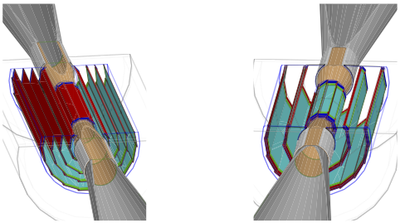
\includegraphics[width = 10 cm]{Pictures/vxd/ild_VXD.png}
     \caption{Overview of the two vertex detector option for the ILC. On the left, it is made of five single sided layers, whereas the right one represents three double-sided layers.}
   \end{figure}
   
   %They are two different geometrical designs understudied to build the \gls{VXD}. 
   %The first idea is to have a \gls{VXD} with five single-sided layers with a radii range from 15 to 60 mm.
   %The other option is to have three double-sided layers, which will have pixel sensors on both sides separated by a mechanical structure of 2 mm thickness. 
   %The radii range is from 16 to 60 mm.

   Both geometry designs are based on  pixel sensors instead of strips detectors.
   A non-exhaustive list of the possible technologies are presented below:
    
   \subsubsection{FPCCD}
   
     The \gls{FPCCD} \cite{CalanchaParedes} is based on the \gls{CCD} processes.
     The sensor is using small pixels size (approximately $\sim 5 \mu\text{m}$) to provide a sub-micron spatial resolution and an excellent capability to separate two nearby tracks.
     Its thickness is 50 $\mu\text{m}$ and the epitaxial layer (15 $\mu\text{m}$ thick) is completely depleted to limit the charge spreading around pixels and to reduce the number of hits per pixel.
     However, the \gls{CCD} architecture provides slow readout and the matrix will be read between consecutive bunch trains, helping to reduce the power consumption and avoiding beam induced RF noise.
     The \gls{FPCCD} are planned to be operated at $-40 \degres$C.

   \subsubsection{DEPFET}
    
    The \gls{DEPFET} \cite{Richter2003} is an \gls{APS} in which field effect transistors are incorporated into each pixel.
    The single point resolution is $\sim 3$ $\mu\text{m}$ for pixels with a size of 20 $\mu\text{m}$.
    The silicon itself is used as sensitive part but also as a mechanical structure, minimising the support and services.
    The sensor is completely depleted of free charged carries thanks to a voltage applied to the thickness.
    The rolling-shutter approach is used for reading each row and the column readout is done by two auxiliary \glspl{ASIC}.

    The \gls{DEPFET} technology is the one chosen  to build the vertex detector of the BELLE-II experiment\cite{depfetBelleII}.

    %Rapid and efficient collection of signal on a deep implant underneath the field effect transistor
    %Inside pixel: first amplification of signal
    %Columns readout by two auxiliary \glspl{ASIC} while rows read out in rolling shutter mode.

   \subsubsection{CMOS}

   Different options for \gls{CMOS} pixel sensors are studied, such as the 3D integrated \gls{CMOS}, but due to the context of this thesis, the work will focus on the \gls{CMOS} sensors based on the \gls{MIMOSA} architecture developed by the IPHC of Strasbourg. 
   This technology is described in section~\ref{sec:CMOS}.
  % The STAR experiment at RHIC is the first one to get an entire vertex detector made of ULTIMATE-MIMOSA28 CMOS sensors.
   %One of the technology developed is described in section~\ref{sec:CMOS}.

   For all the technologies, the sensors' power consumption has to be minimised in a way to reduce the cooling system and in the same time the added material budget in the sensitive detector volume.
   As it was shown on the figure~\ref{fig:bunches} of the chapter~\ref{chap:ILC}, the bunch train will last less than 1 ms for a dead time of 200 ms.
   Two possibilities are envisaged to benefit from the beam structure.
   The first one consists to store the hits information thanks to a time stamp during the bunch crossing and to read out the data after the last collision.
   This method might be used by the \gls{FPCCD} technology due to the slow integration time of the \gls{CCD}.
   Another solution is to use power-pulsing.
   Right after the last collision, the sensors are switched off or the power consumption is reduced as mush as possible, and before the first collision, the sensors is switch on again.
   This pulsing method is studied by different collaborations. 
   
   Another aspect not discussed yet is the radiation tolerance of the detector, which is directly related to the beam background.
   The first layer is the most affected by the background and it should have a high radiation tolerance. 
   The required radiation tolerance is about 1 kGy for the total ionising dose and a fluence of $10^{11}\text{n}_{eq}\text{/cm}^2$\cite{Behnke2013}.

   The efficiency of the \gls{VXD} has also to be excellent in order to maximise the tracking performances.
   The efficiency is defined here as the ratio of detected particles over all the particles crossing the detector.
   If one layer of the vertex detector misses a hit, the track reconstruction will be less accurate 
   
   % the vertex detector optimisation can be only achieved by taking into account the beam structure.
   %As it was shown on the figure~\ref{fig:bunches} of the chapter~\ref{chap:ILC}, the bunch train will last less than 1 ms for a dead time of 200 ms.
   %Instead of reading the data during the bunch train, the sensors can be read out right after the end of the bunch train, then they can be switched off, or reduce their consumption as mush as possible, and they can be switched on at their nominal working value right before the first collisions. 
   %This dead time can also be used to cool down the system.
   %Indeed, the cooling system add an additional material 
  
   
   

   \todo{Cooling system, integration time, radiation tolerance, electromagnetic interference}

   To summarise, the expected parameters expected for the \gls{ILC} are: 
   \begin{itemize}
     \item An excellent impact parameter resolution: $ a \sim 5 \mu\text{m}$ and $b \sim 10 \mu\text{m}$
     \item A material budget not exceeding 0.1 \% $X_0$ per layer for the single-sided option (0.16 \% $X_0$ for the double one)
     \item Radius of the first layer $\sim$ 15/16 mm
   \end{itemize}

  \section{PLUME}

  The \acrfull{PLUME} project aims to produce double-sided ladder prototypes with respect to the \gls{ILC} requirements\cite{PLUME}.
  Three labs in the Europe are involved: the IPHC-PICSEL in Strasbourg, the University of Bristol and DESY in Hamburg.
  The collaboration is studying the feasibility to build such vertex detector using \gls{MAPS} thinned down to $50 \mu\text{m}$ and is exploring the benefits of this design.
  Strasbourg is in charge to develop and mount the sensors on the modules, to take care of the readout and the \gls{DAQ}, and to provide a cooling system.
  The mechanical design, stability measurements and building the ladders are done by the University of Bristol, while DESY has studied the ladder mock-up, performed power-pulsing tests and is now characterising and validating the modules in the lab.
  In 2016, DESY has provided the opportunity to test the ladder in real conditions thanks to the test beam facility and the possibility to use the \gls{DAQ} software developed at DESY: EUDAQ\todo{REF: EUDAQ}.

    \subsection{Design and goals}

    The figure~\ref{fig:PLUME} illustrates the design of a PLUME ladder.
    The ladder structure is defined by the sensors arrangement on the mechanical structure (positioned next to each other).
    In this design, the stiffener is a 2 mm thick \gls{SiC} foam which has a density varying between 8 \% and 4 \% (depending on the ladder version) and could be reduced to only 2 or 3 \%.
    %The mechanical structure is made of a 2 mm thick silicon carbide foam which has a density varying between 8\% for the prototype build before 2011 and 4\% for the new ones.
    The choice of this foam is a good compromise between the stiffness and the thickness compare to other materials. \todo{REF Joel paper}
    The figure~\ref{fig:SiC} is representing the structure of this foam.
    It is macroscopically uniform and has the advantage to be easily machinable.
    Nevertheless, it has a low thermal conductivity (50 W/m/K) and can't be used to dissipate the heat.
    On each side, a low mass flex-cable is glued, which is used to connect the sensors for powering and managing them.
    It is made of copper traces coated in Kapton, but new prototypes using aluminum traces are developed and currently tested in order to reduce the material budget.
    %It is made of copper traces (prototype before 2011) or aluminum traces (new prototypes) coated in Kapton. 
    The ladder embeds twelve sensors, six on each face, that are glued and connected to the flex cable.
    On one edge of the flex-cable, a single \gls{ZIF} connector is used to link the ladder to the external board servicing, via a jumper cable.
    For the moment, the design is dedicated to the MIMOSA-26 sensors thinned down to $50 \mu\text{m}$ but it can be adapted to any kind of \gls{MAPS} sensors having the same thickness. 
    Although the MIMOSA-26 has a spatial resolution better than 3$\mu$m (see subsection~\ref{subsec:Mi26}), the integration time is not suited for the bunch train structures of the \gls{ILC}.

    The aims of the collaboration are to build ladders with a material budget better than 0.35\% of $X_0$ for a spatial resolution better than 3$\mu$m, and thus to evaluate the benefits of a double-sided measurement.

    \begin{figure}[!h]
      \centering
      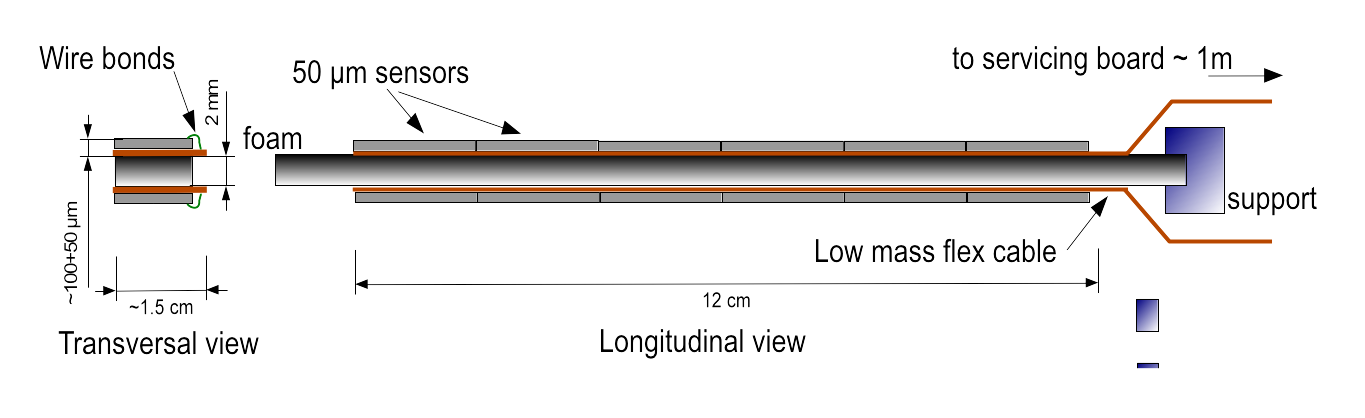
\includegraphics[width = 15 cm]{Pictures/vxd/plume_finalGoal.png}
      \caption{Side view (transversal and longitudinal) of the PLUME mechanical structure.}
      \label{fig:PLUME}
    \end{figure}

    \begin{figure}[!h]
      \centering
      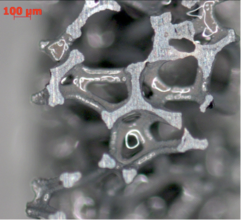
\includegraphics[width=0.3\textwidth]{Pictures/vxd/foam2.png}
      \caption{Microscopical view of the silicon carbide foam structure.}
      \label{fig:SiC}
    \end{figure}

    \subsection{Prototypes}

    Since 2009, the collaboration is studying the design, the production, the impact of the mechanical structure on the ladder's performances, but also how to power and control the sensors together.
    The first ladder prototype, called version-0 (V-0) was developed and tested in 2009.
    The purpose of this prototype was to settle the fabrication and the test beam procedures, without trying to reach the desired material budget goal.
    Two MIMOSA-20 analog output sensors were mounted on each side of a stiffener, providing a $1 \times 4 \text{ cm}^2$ sensitive area.
    The prototype was tested in 120 GeV pion beam at the CERN-SPS and the results have demonstrated the benefits of the double-sided measurement on the spatial resolution, which is improved by about 25\%\cite{Nomerotski}.

    Then in 2010, a second prototype featuring a design closer to the wanted goal, called version-1 (V-1), was developed.
    Each module of the ladder was made of Kapton flex-cable with a thickness of 0.14 mm, using copper traces.
    They are denoted \gls{OKF}, where Optiprint is the vendor of these flex-cable.
    It is the first version to embed six MIMOSA-26 binary output sensors working simultaneously on each side of the stiffener.
    The material budget is estimated to be 0.65 \% of $X_0$ in the sensor's sensitive area. 
    The aim of this prototype was to validate the operation of multiple sensors in a chain.
    Two ladders were tested in real conditions.
    The first one was tested with 120 GeV pions at CERN-SPS in 2011, while the second ladder was tested in April 2016 with up to 5 GeV positrons at DESY in Hamburg. 
    The DESY test beam results are presented in chapter ???, while a specific study of the sensor's deformation observed at CERN is discussed in chapter ???.

    \begin{figure}[!h]
      \centering
      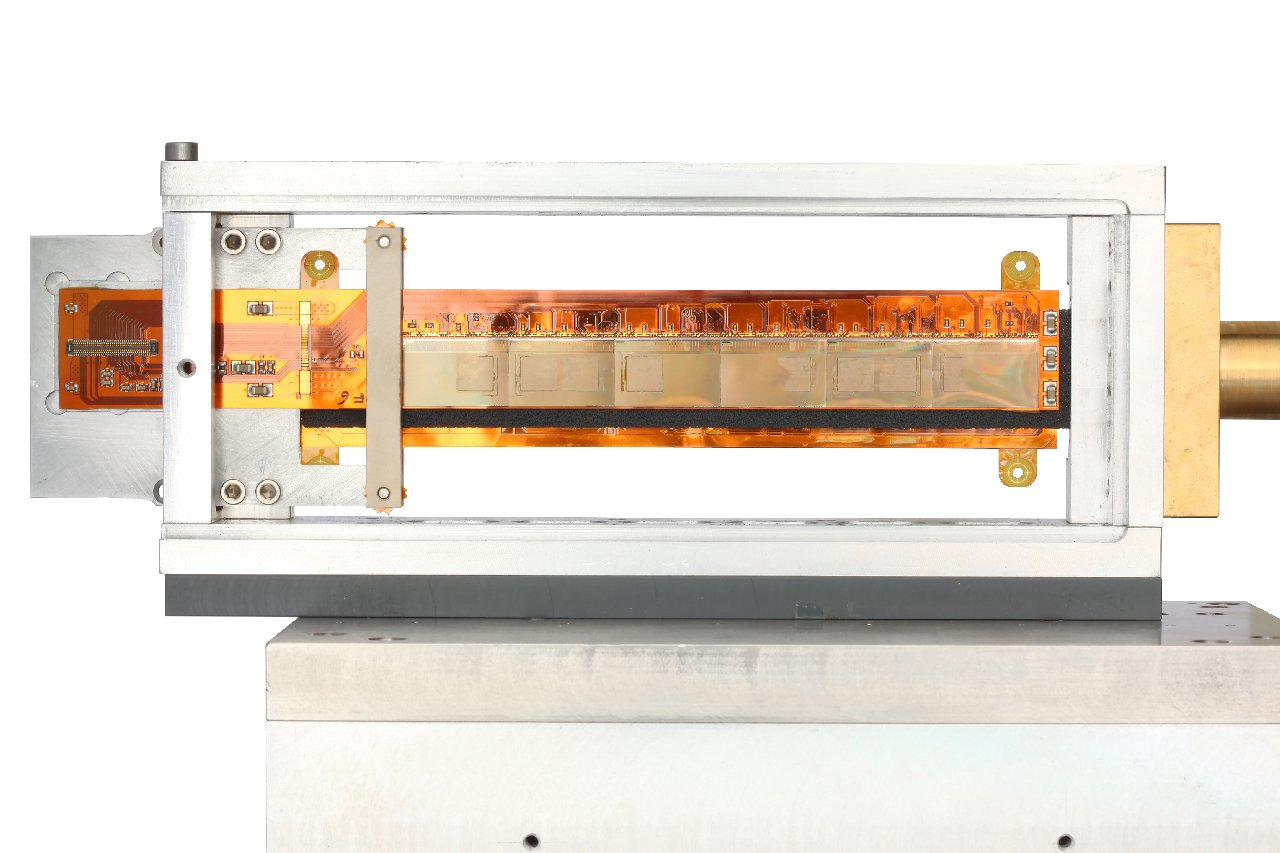
\includegraphics[width = 12 cm]{Pictures/vxd/plume_ladder2010_frontView}
      \caption{Front view of the ladder version-1 made in 2010 in its holding box. On the left, there is the connector to the output board servicing, on the right a connection to blow air on the module. As this version was not made with a mirrored design, the flexible cables are not entirely overlapping and the SiC foam can be seen (in black here).}
    \end{figure}

    At the beginning of 2016, the third prototype versions were mounted but have not yet been completely tested.
    In fact, this new version is divided into two sub-versions: one using copper traces and the other one aluminum traces.
    Nevertheless, both sub-versions have a new design featuring reduced traces thickness to have a narrower flex-cable (18 mm width) adjusted to the sensors width in order to minimise the dead areas.
    The flex-design has slightly changed to have a mirrored geometry (figure~\ref{fig:AM01}) and a straight geometry in order to minimize the dead area too and have a better alignment solution.
    The stiffener is made of a lower density \gls{SiC} foam reducing the global material budget. 

    \begin{figure}[!h]
      \centering
      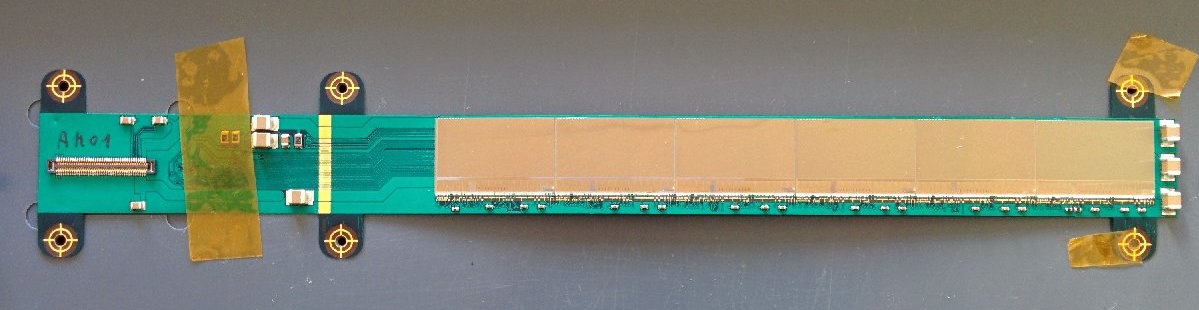
\includegraphics[width = 12cm]{Pictures/vxd/AM01.jpg}
      \caption{Picture of the first mirrored module made with aluminum traces. The cable width is adjusted to the size of the sensor.}
      \label{fig:AM01}
    \end{figure}
    The table~\ref{tab:X0} summarises the material budget reached by the different prototypes.

    %Before to reach the lightest ladder with a material budget of only 0.35 \%, the collaboration has studied the design, production and impact of the mechanical structure, but also how to power and control the sensors.
    
    %%The first ladder prototype (here labeled V0) was developed and test in 2009.
    %It has two MIMOSA-20 analog output sensors on each side of a stiffener, providing a $1 \times 4 \text{ cm}^2$ sensitive area.
    %As the purpose of this prototype was to settle the fabrication and the beam test procedure, the sensors and the flex-cables were not optimised.
     
    %The second prototype featuring the final device design (V1) was developed in 2010. 
    %The material budget is estimated to be 0.65 \% of $X_0$ in the sensor's sensitive area. 
    %It is the first version to embed six MIMOSA-26 binary output sensors on each side of the stiffener that were working simultaneously.
    %Two ladders were tested, one with 120 GeV pions at CERN-SPS in 2011 and the second one with positrons up to 5 GeV at DESY.
    %The test beam at DESY is presented in chapter ... and some results of sensor's deformation observed at CERN are discussed in chapter ...

    %The third prototype was mounted at the beginning of 2016 and has not been yet tested. 
    %The traces thickness was reduced, the flex-cable width was adjusted to the sensors width and the stiffener was made of a lower density Silicon Carbide foam reducing the material budget and the dead areas.

    \begin{table}
      \begin{center}
        \begin{tabular}{c c c c c c c}
        \hline %----------------------------
        \multirow{2}*{Layer}  & \multicolumn{3}{ c }{budget (\% X$_0$)}  \tabularnewline
                              &  V-0 & V-1 & Goal \tabularnewline
        \hline %----------------------------
        \hline %----------------------------
        Sensor                & 0.053 & 0.053 & 0.053 \tabularnewline
        Flex-cable            & 0.524 & 0.150 & 0.034 \tabularnewline
        Passive components    & 0     & 0.033 & 0.033 \tabularnewline
        Stiffener (foam)      & 0.764 & 0.175 & 0.087 \tabularnewline
        \hline %----------------------------
        \textbf{Total}        & 1.926 & 0.654 & 0.334 \tabularnewline
        \hline %----------------------------
        \end{tabular}
        \caption{Estimation of the material budget for the different prototypes of the PLUME ladder.}
        \label{tab:X0}
      \end{center}
    \end{table}

    \subsection{Perspectives}

    Although the collaboration has shown their expertise to build light mechanical structures, more tests and optimisations have to be done.
    MIMOSA-26 sensors are not designed to match the \gls{ILC} specs. 
    The integration time of this sensor is 115.2 $\mu$s, whereas the bunch train last only 0.95 ms (bunch crossing spaced out by 337 ns), a new CPS with a faster integration time has to be integrated.
    Another problem of the MIMOSA-26 sensors is that they are not suited for a power pulsing. As a reminder, the principle of the power pulsing is to reduce the consumption of the sensor during the 200 ms dead time. 
    Nevertheless, a power-pulsing study on a single Mi-26 sensor has been done and the results have shown that the nominal supply voltage of the MIMOSA-26 can be lowered from 3.3 V to 1.85 V without losing the sensor's registers. 
    The fake hit rate measured was close to the one obtained in  normal conditions after the sensor reaches a stable operation.
    Moreover, the power consumption was reduced by a factor 6.34\cite{Kuprash2013}. 

    A complete power-pulsing study of the whole ladder in the lab has to be done in order to make sure that the sensors are still behaving correctly.
    If the first results are comforting, the power-pulsing will be tested under real conditions with a high magnetic field.
    The impact of the Lorentz forces due to the coupling of the power-pulsing and the magnetic field is going to be studied, especially is this structure will induce unwanted deformations or vibrations. 

    The collaboration is considering to embed the sensors directly inside the multi-layer micro-cable\cite{Baudot2012}.
    The chips are glued on the first polyimide substrate layer, then the metal layer is deposited on top of it and the metal traces are directly connected to the chips pads.
    Then an insulator is added to the module.
    The advantages of this technique are, firstly, the direct connection of metal traces to the pads that avoid wire-bonding and can reduce, at the same time, the width of the module.
    And secondly, this structure has the advantage to apply the mechanical stress on the polymer wrapping, thus reducing it on the sensor.

    A closer perspective for the collaboration is to integrate two ladders in the physics commissioning of the BEAST experiment at KEK.
    The version-2 ladder will be used but a second option is foreseen.
    MISTRAL sensors will be mounted on the flex-cable instead of the MIMOSA-26.
    These sensors have a bigger sensitive area, a faster integration time  ($\sim 20\mu\text{s}$) but a worth spatial resolution ($< 10 \mu\text{m}$) due to the pixel size (pitch of $36 \text{x} 62.5 \mu\text{m}^2$).

  \section{Integration of CMOS sensors}
  \label{sec:CMOS}

  %Since the beginning of the 1990's, a new alternative to the \gls{CCD} was developed by the imaging industry: the \gls{APS}.
  %They have produced thanks to the \gls{CMOS} industrial process and are equipping nowadays the sensors of the camera.
  %They are called so because the pixel is made of a photodiode associated with an active amplifier.
  %They are called active pixel sensors because the pixel is made of a photodiode  and an active amplifier. 
  %This technology is well used in the industry and equipped most of the camera produced.

  The PICSEL group of the IPHC at Strasbourg is developing since 1999 CMOS sensors called MIMOSA for \textit{Minimum Ionizing MOS Active pixel sensor}. 
  They are semi-conducting pixel sensors based on the \gls{APS}, an alternative to the \gls{CCD} developed at the beginning of the 1990's by the imaging industry and used nowadays for the smartphone's cameras.
  One particularity of the sensors developed by Strasbourg is that the different region of the \gls{CMOS}, such the sensitive area or the electronic layer where the signal is processed, are made of the same material.
  This device is called then \acrfull{MAPS} and the different layers are:
  \begin{itemize}
    \item A substrate providing a mechanical stability;
    \item An epitaxial layer which is the sensitive volume of the sensor;
    \item An electronic layer where are located the diodes collecting the charges and the microelectronic processing the signal.
  \end{itemize}

  The motivation to use this technology or any other silicon sensor in particle physics is due to the minimum energy needed to create an electron/hole pair by a traversing particle.
  In silicon, this minimum energy is only 3.6 eV, while for a gaseous detector, it is close to 30 eV.
  %The first sensor developed by the PICSEL group of the IPHC of Strasbourg was born in 1999.
  %It was the first sensors prototype for physics of the PICSEL-family, called MIMOSA for \textit{Minimum Ionizing MOS Active pixel sensor}.
  %They are \gls{MAPS} because the sensitive

  %The PICSEL group of the IPHC of Strasbourg is developing \gls{MAPS} for the particle physics community since 1999.
  %They are called monolithic because the sensitive volume and the microelectronic circuitry form one physical block.
  
    %\subsection{Principle of a CMOS sensor}

    %When a particle is traveling through matter, it loses energy via interaction with electrons and nuclei.
    %For a thin layer of material, particles can cross all of the environment and lose a small fraction of their energy.
    %It is admitted that \gls{MIP} creates 80 electrons per microns. 
    %For thin layer, energy loss is described by a Landau while thick material by a Gaussian.

    \subsection{Charges creation and signal collection}   

    The \gls{CMOS} sensor can detect crossing particles thanks to their structure, but also to the interaction of particles with matter.
    When a particle is traversing a layer of matter, it loses energy via interactions with electrons and nuclei.
    Due to the size of a \gls{MAPS}, it loses only a small fraction of its energy, and the energy loss can be described by a Landau.
    A \gls{MIP} creates 80 electrons per microns inside the silicon.

    At the beginning, the microelectronic industry has insulated the transistors from the substrate thanks to a high resistivity layer, called the epitaxial layer.
    The development of \gls{CMOS} sensors was accelerated due to the properties offered by these semiconductors.
    
    %The different structure of the sensor has distinct doping.
    %The bulk is a P++ doped layer made with a moderate quality silicon.
    %The crystal structure has many defects leading to a high rate recombination of charge carriers.
    %Above the substrate, the epitaxial layer is P- doped and made of a good quality silicon.
    %The electron/hole pairs created in this layer do not recombine instantaneously like in a highly doped layer but they are thermally diffused. 
    
    The \gls{CMOS} sensors developed by the IPHC at Strasbourg are called monolithic \gls{MAPS} sensors because the different layers of the sensor are made in one block of the same material, but with different doping.
    The structure of the sensor is a highly doped P+ substrate made of a moderate quality silicon. 
    The crystal structure contains a lot of defects, hence the recombination rate of charge carriers is high.
    Above the bulk, a low-doped P- layer is grown.
    The silicon used has a good quality, thus the charge carriers have less chance to recombine.
    It is the sensitive part of the sensor and is called the epitaxial layer. 
    On top of it, an N-well implant has the role of the charge collection.
    The interface between the N-wells and the epitaxial layer forms a P-N junction called a collection diode.
    A depleted area is created by this junction, on which the charge carriers are attracted.
    Nevertheless, this P-N junction is only one part of the pixel.
    Next to the N-well implants are sitting highly doped P-well in charge to reflect the charge carriers to the implants.
    The difference of doping between the bulk and the epitaxial layer is also used to reflect the charge carriers to the collection diode.

    The typical doping concentration are $10^{15} \text{at/cm}^3$ for the epitaxial layer, $10^{19} \text{at/cm}^3$ in the substrate and $10^{17} \text{at/cm}^3$ for the other layers.
    The doping concentration defines the size of the depleted region.
    For this doping concentrations, only a small region around the P-N junction is depleted, while the epitaxial layer is mainly undepleted. 
    As no external voltage is applied to the sensor to increase the depleted region, the charge carriers created by crossing particles are thermally diffused into the epitaxial layer to the diode.
    Nevertheless, the different doping levels produce a built-in voltage defined as: 

    \begin{equation}
      V_b = \frac{kT}{q}ln\left( \frac{N_{p+}}{N_{p-}}\right)
    \end{equation}
    
    The built-in voltage depends on the Boltzmann constant $k$, the temperature $T$, the elementary charge $q$ and the different concentrations doping $N_{p\pm}$ of the interface.
    Due to the different doping levels, the electrons are restricted to diffuse inside the sensitive volume, to be then guided towards a collection diode.
    One effect of the thermal diffusion is that the average path of the electrons in the epitaxial layer is longer than the one they would have in a fully-depleted sensor.
    Hence, the probability of recombination between an electron and a hole is increasing.
    Also, the charges tend to spread more around neighboring n-well.
    Therefore, the charge collection efficiency is lower than the fully-depleted sensor.

    \begin{figure}[!h]
      \centering
      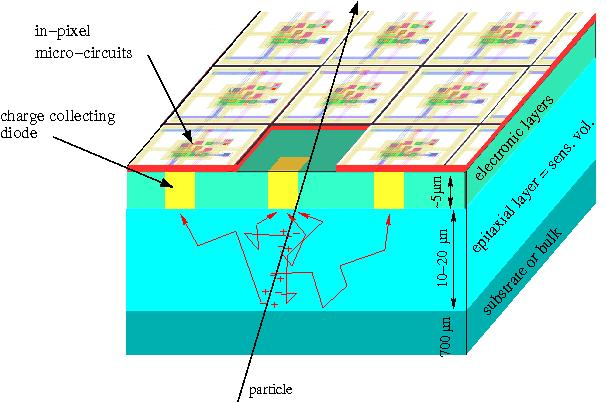
\includegraphics[width = 10cm]{Pictures/vxd/principeMapsMIP.jpg}
      \caption{Drawing of MAPS structure representing the different layers of the sensor and the path of charge carriers in the epitaxial layer.}
      \label{fig:principleMaps}
    \end{figure}

    \subsection{Pros and cons of the technology}

    The \gls{CMOS} sensors have several interesting properties.
    First of all, the fabrication cost is lower than other pixel technologies due to the industrial processes used to build the sensors.
    Therefore, many prototypes and bigger matrices can be built, while benefiting from the industrial experience.
    For example, the imaging industry has developed smaller and smaller grid size and a pitch size of ten microns can be achieved.
    
    Secondly, due to the size of the depleted area, the charge carriers tend to spread more over neighboring pixels.
    On the one hand, the signal collected per pixel is smaller, but on the other hand, the reconstruction of the hit position with a centre of gravity algorithm is improving the spatial resolution.
    To give an idea, a binary output sensor with a pitch of 18.4 $\mu\text{m}$ can achieve a spatial resolution better than 3 $\mu\text{m}$.

    Thirdly, the distinct doping of the different layers is responsible for the reflection of the charge carriers to the collection diodes.
    However, only the interface between two different doped regions is responsible for this reflection.
    Thus, the substrate can be thinned down to few microns leading to a sensor with a thickness of 50 $\mu\text{m}$, while keeping the possibility to manipulate them.
    In this way, the material budget can be reduced down to 0.053\% $X_0$.
    %The bulk is not entirely responsible for the charge carriers reflection, only the interface between the substrate and the epitaxial layer is mainly responsible for the reflection.
    %The substrate can be thinned down to few microns leading to a sensor with a thickness of 50 $\mu\text{m}$ while keeping the possibility to manipulate them.
    %The material budget can then be reduced to 0.053 \%.

    Nevertheless, the thickness of the epitaxial layer (usually between 10 and 15$\mu$m) and the small depleted region are responsible for a small charge collection.
    As a matter of fact, a \gls{MIP} is creating 80 electron/hole pairs per microns, so the number of charges collecting by the diode is of the order of a thousand electrons.
    Hence, the signal created is only a few millivolts and low noise electronics have to be used for processing the signal.

    CMOS sensors are sensitive to ionizing and non-ionizing radiations that degrade the sensor properties.
    The non-ionizing radiations are damaging the crystal structure of the epitaxial layers, creating defaults in the lattice.
    The recombination rate is increasing and reduces the signal collected.
    To avoid this effect, two solutions are possible.
    The first one is to reduce the size of the pixels in order to decrease the path of the particles from the epitaxial layer to the collection diodes.
    Nevertheless, the cost to build sensors with a smaller pitch is increasing.
    The second solution is to increase the resistivity of the epitaxial layer to expand the depleted area.
    
    The ionizing radiations are responsible for charges accumulation in the electronic layer.
    The leakage current is increasing in the pixel and diode collection.
    To reduce the leakage current, smaller diodes can be used to reduce the impact of the leakage current but as it was explained before, the cost of fabrication is increasing.
    
    \subsection{Signal processing}

    If no charge is collected by the pixel, the voltage at the equivalent capacitor of the diode is evolving because of the leakage current inherent in the junction.
    The pixel reading can be done in two different ways, depending on the method used to minimise the leakage current effect.
    Currently, two pixel's architectures are used to compensate the diode's leakage current: the \textit{3 Transistors pixel design}, mainly used in imaging, and the \textit{self-biased pixel design}.
    The circuit diagram which is shown on the figure~\ref{fig:elecArch} represents the two methods to design pixel.

    The first one, presented on figure~\ref{fig:3T}, consists to reinitialise the collection diode's voltage to a reference voltage thanks to a \textit{reset} transistor, denoted M1 on the diagram.
    This method works in two steps. 
    Firstly, the M1 transistor is closed and the charge of the equivalent capacitor $C_d$ associated to the junction P-N, represented by a diode on the diagram, is slowly decreasing because of the diode's leakage current. 
    During this phase, the pixel is sensitive and is read.
    After a time interval equivalent to the integration time of the sensor, the transistor M1 is opened to recharge $C_d$ to its initial voltage.
    During this time, the pixel is not sensitive.
    While M1 is used for the reset, M2 is used as a pre-amplifier of the signal created by the diode and M3 link up the voltage to the output of the circuit.
    Although this compensation method is fast, it generates a dead time for detection between two readings.
    
   % The first method consists to force time to time the reinitialisation of the voltage on the collection diode leads to a reference value thanks to a \textit{reset} transistor.
   % In order to limit the impact of the noise created by thermal fluctuations during the reinitialisation, a \textit{correlated double sampling} is used. A first voltage reading from the output of the pixel stores the \textit{reset} level and a second reading subtracts the measured voltage previously read to reduce the noise impact.
   % Although the compensation is fast, it generates a dead time for detection between two readings.
    
    The figure~\ref{fig:selfBiased} depicts the \textit{self-biased pixel design} method\cite{Deveaux2009}.
    It is using a P-N junction (symbolised here by a diode mounted on the other side) coupled to the N-well implant to absorb the leakage current.
    The inverted diode is continuously compensated the diode's leakage current, thus the dead time vanishes.
    %Using a forward p-n junction has the advantage to avoid any dead-time because the diode's leakage current is continuously compensated by the second diode.
    While no particle is crossing the sensor, an equilibrium appears between the leakage and recharge current.
    A particle going through the sensor disrupts this equilibrium.
    The charges collected by the pixel lead to a discharge of the diode's capacitor $C_d$, followed by a recharge of this capacitor thanks to the second diode to reach again the equilibrium.
    %When a particle is crossing the sensor, the charges are collected by the pixel, leading to a discharge of the diode's capacitor $C_d$, which is followed by a recharge to reach again the equilibrium.
    Nevertheless, if the recharge procedure is too fast compare to the integration time, the physics signal is masked and the passage of the particle is never notified.
    %Nevertheless, the recharge procedure should be slower than the integration time to be able to detect physics signal during detection.
    %Indeed, when the recharge is too fast, the physics signal is masked and the passage of particle will never be notified.
    Even if the time interval to recharge the capacitor $C_d$ is set properly, an important charge collection per pixel could disturb the recharge phase and the pixel will reach a stable level again only a long time interval of the order of 10 ms.

    \begin{figure}[!h]
    \centering
    \begin{subfigure}[t]{0.45\textwidth}
        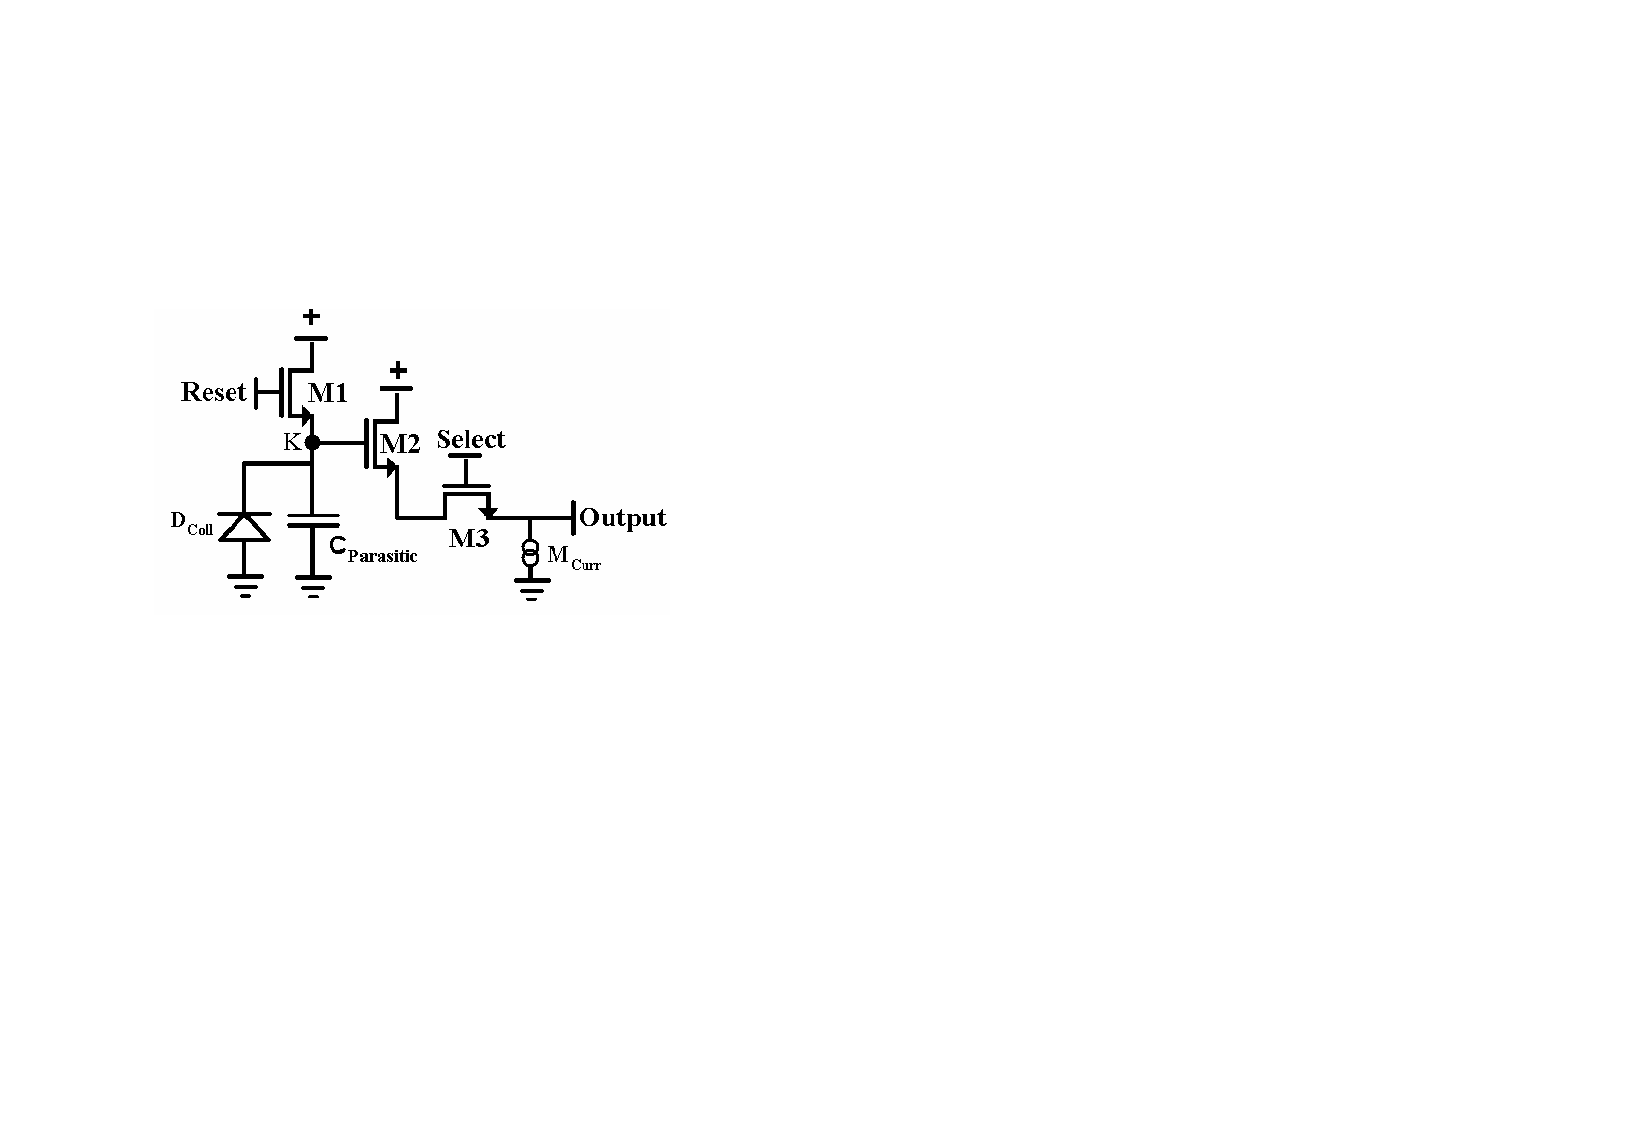
\includegraphics[width=\textwidth]{Pictures/vxd/3T_architecture.pdf}
        \caption{Three transistors (3T) pixel design.}
        \label{fig:3T}
    \end{subfigure}
    ~%\quad
     %add desired spacing between images, e. g. ~, \quad, \qquad, \hfill etc. 
      %(or a blank line to force the subfigure onto a new line)
    \begin{subfigure}[t]{0.45\textwidth}
        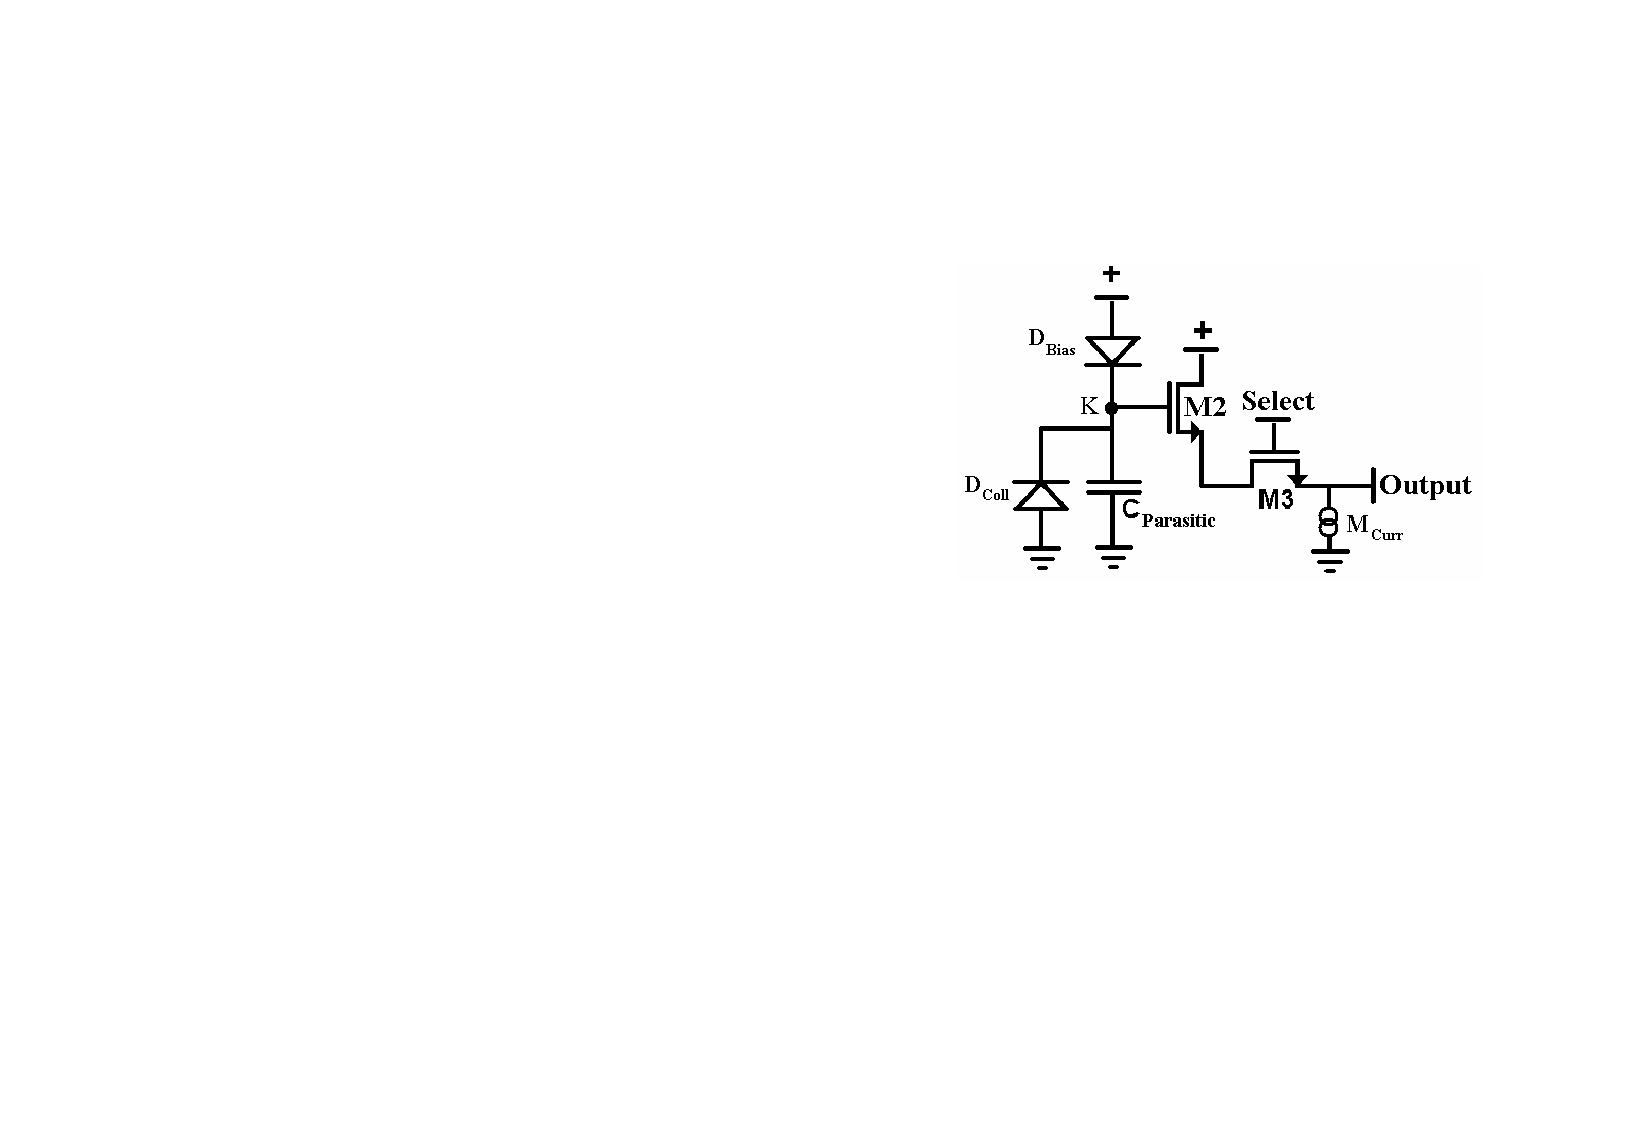
\includegraphics[width=0.95\textwidth]{Pictures/vxd/self-biased_architecture.pdf}
        \caption{Self-biased pixel design.}
        \label{fig:selfBiased}
    \end{subfigure}
      \caption{Two different architectures of pixel.}
      \label{fig:elecArch}
    \end{figure}    

    \subsubsection{Integration time and readout}

    For a non-depleted epitaxial layer, the charge carriers are thermally diffused to the collection diodes.
    The time to collect these charges in a pixel is $\sim$ 100 ns, setting a maximal limit to read the signal.
    This integration time is not reachable due to other factors, like the pixel occupancy or the time needed to obtain the information of all the pixels.
    Also, a compromise to reach fast integration time has to be done.
    Faster is the sensor, more important is the power consumption of the electronic.
    Moreover, to reduce the integration time, a solution consists of increasing the size of the pixels.
    In consequence, the pointing resolution of the device is impacted.
    For the case of the \gls{ILC}, the integration time is dictated by the pixel occupancy that should not be bigger than a percent, to stay in the using sensor's range and to be able to reconstruct the impact.

    The first sensors developed were using an analog output.
    With this approach, the pixels were addressed sequentially and their output was multiplexing in one bus line.
    The advantage of such method is that the discrimination can be adjusted offline for each pixel, thus compensating the nonuniform response.
    Nevertheless, the integration time is depending on the operational frequency of the bus (usually 50 MHz) and the number of pixels contained in a matrix.
    For a sensor having millions of pixels, the integration time is then of the order of the millisecond.
    An analog output is then too slow for a \gls{ILC} purpose. 
    
    \begin{figure}[!h]
      \centering
      \missingfigure{Rolling shutter}
      \caption{Parallel column readout.}
      \label{fig:rollShut}
    \end{figure}
    
    To overcome this problem, an approach is to group the pixels in columns and to read them in parallel.
    The figure~\ref{fig:rollShut} depicts the principle of this method called \textit{column parallel readout} or \textit{rolling-shutter}.
    Instead of having one bus line for the whole matrix, each column has its own bus and a data sparsification logic is integrated on the periphery of the sensor.
    One row is read out between 100 ns and 200 ns, independently to the number of pixels contained in it.
    In consequence, a matrix containing thousands of rows has an integration time of $\mathcal{O}(100\mu$s).
    Moreover, to increase the integration time an output memory is duplicated at the periphery of the sensor.
    Hence, when one line is read, the precedent one is processed by the electronics at the end of each bus line of each column.
    To minimise the data bandwidth, only the pixels above certain thresholds are read thanks to discriminators coupling to a zero suppression logic, called \gls{SUZE}.
    In this way, only the address of the first pixel hit in a row and the number of the adjacent fired ones are stored.
    This memory is duplicated to be able to process one row, while the previous one is read out by the outside world.
    In order to increase the readout speed, two techniques are conceivable\cite{Winter:2009zz}.
    The first one provides elongated pixels in the vertical direction in order to reduce the number of rows, thus degrading the spatial resolution in the same direction.
    The second one consists of dividing the columns into two distinct parts, which have its dedicated output.

    %When one line is read, the precedent line is processed by the electronics on the bottom each column.
    %Only the pixels having a signal above certain thresholds are read.
    %A zero suppression logic, called \gls{SUZE}, is in charge to determine the number of fired pixels in a raw and to send the address of the first pixel hit and the number of adjacent ones hit, as shown on figure~\ref{fig:SUZE}.
    %The sequence of fired pixels feed one output memory, while a second memory is read out by the outside world.
    %This technique has the advantage to reduce the data bandwidth.
    %The integration time is then defined as the time to read one line by the number of rows in the matrix.
    %For example, sensors containing a thousand of lines have an integration time of $\mathcal{O}(100\mu$s). 
    %Two techniques can be used to increase the readout speed\cite{Winter:2009zz}.
    %The first one provides elongated pixels in the vertical direction in order to reduce the number of rows, thus degrading the spatial resolution in the same direction.
    %The second one consists of dividing the columns into two distinct parts, which have its dedicated output.

    \begin{figure}[!h]
      \centering
      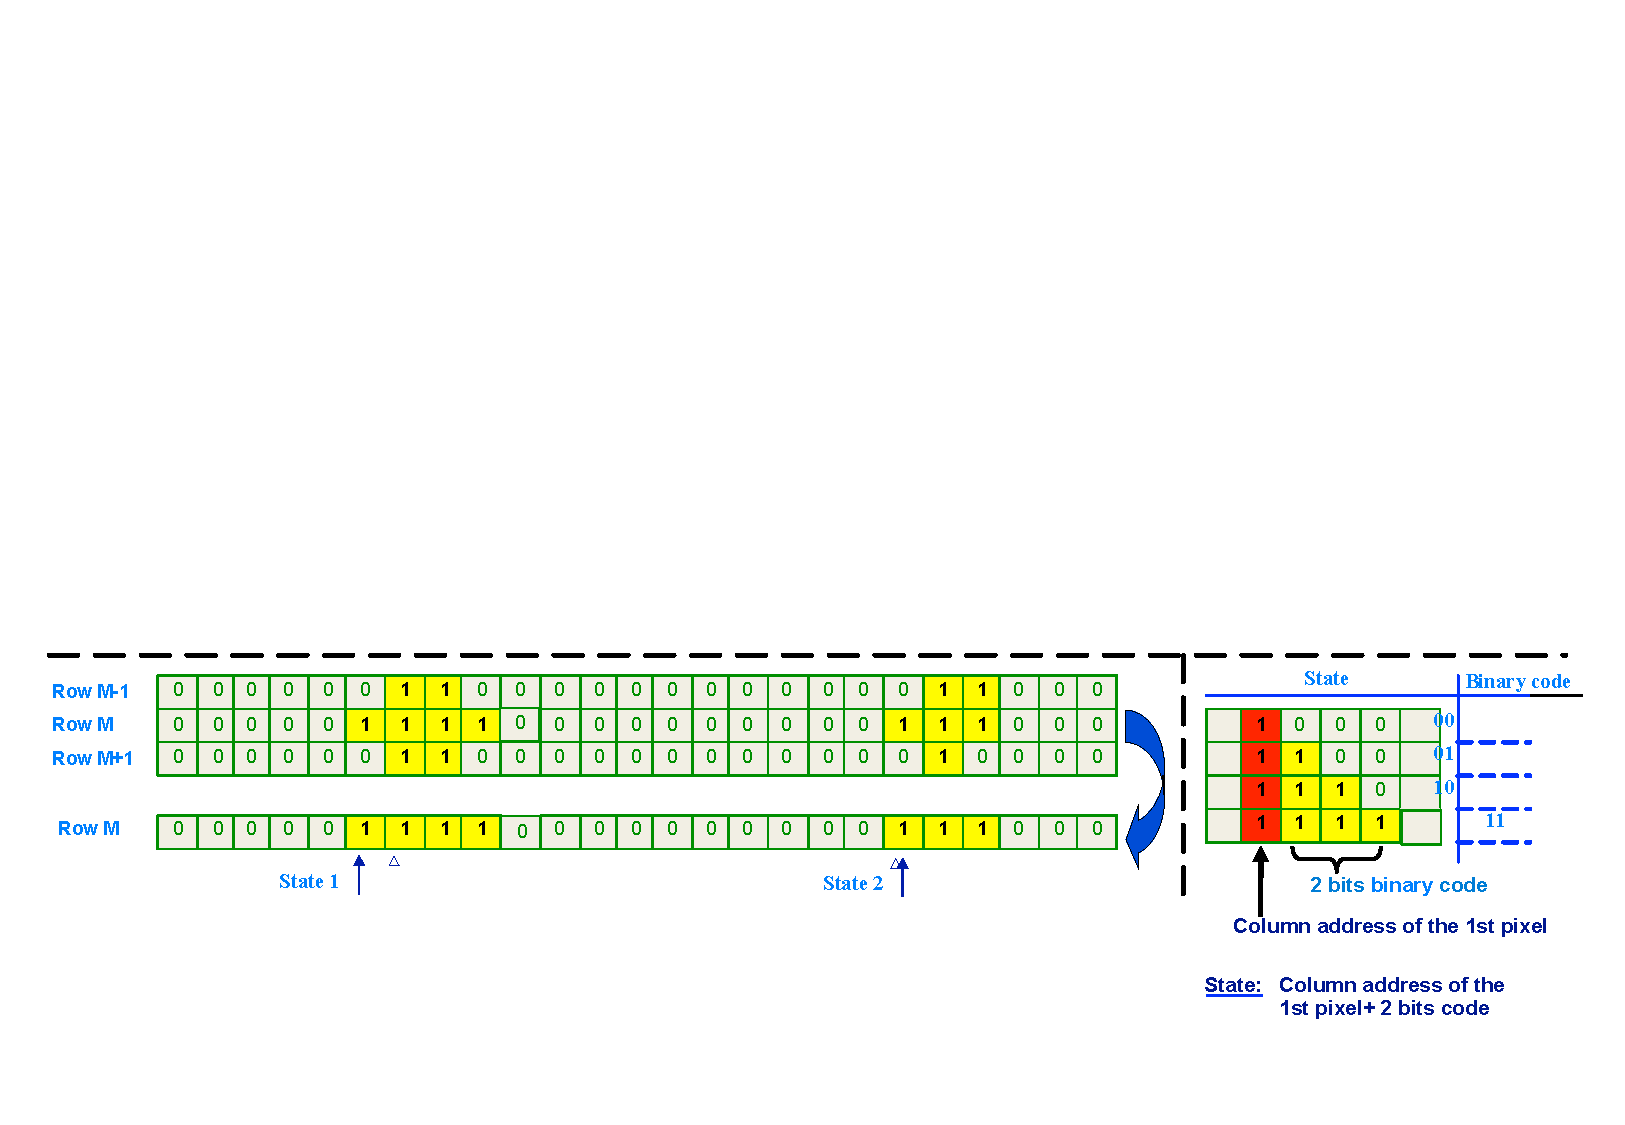
\includegraphics[width=\textwidth]{Pictures/vxd/suze_hit.pdf}
      \caption{Principle of the zero suppression logic. }
      \label{fig:SUZE}
    \end{figure}

    \subsubsection{Noise}

    The \gls{CMOS} sensors are sensitive to the noise.
    Many factors are causing it and the different kind of noise is divided into two categories: the \gls{FPN} and the \gls{TN}.
    The non-uniformity responses of the pixel in a sub-array is responsible for the \gls{FPN} and is regarded as an offset or pedestal, which is subtracted from the pixel response to reduce the impact of this noise.
    The \gls{TN} has different origins, as the shot noise, the pink noise or the thermal noise.
    The different operational phases to read the signal are contributing to the noise.
    
    One contribution to the \gls{TN} appears in the \textit{3T pixel design} only during the reset phase.
    This noise arises when the transistor is open restoring the charge of the capacitor associated with the collection diode.
    It is dependent on the temperature and the diode's capacitance.
    
    The second one is the noise during integration and is caused by statistical fluctuations of the leakage current (shot noise).
    Faster is the integration time, slower is the shot noise contribution.
    
    Finally, the third one arises from the readout, while the column switch and the source follower capacitors are working.
    This noise depends on the contribution of each capacitor.
    
    To remove the \gls{FPN} and the reset noise, a \gls{CDS} is performed inside the pixel or at the bottom of the column.
    It consists to acquire two frames and to subtract the first one to the second one to search for possible signals.
    The chapter~\ref{chap:labTests} describes the steps to characterise the \gls{FPN} and \gls{TN} and to select an appropriate \gls{SNR} in order to minimise the noise contribution, and to find a range on which the sensor is working properly.


    \subsection{State of the art in high energy physics}
    \label{subsec:Mi26}

    \begin{figure}
      \centering
      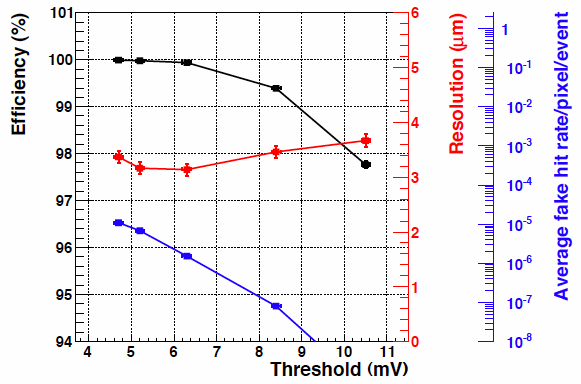
\includegraphics[width=0.8\textwidth]{Pictures/vxd/MIMOSA26_chip26_HR15_20deg}
      \caption{Plots representing the efficiency, the fake hit rate per pixel and the spatial resolution as a function of the discriminator threshold.}
      \label{fig:mi26Perf}
    \end{figure}

    The first full-scale digital sensor developed by the PICSEL group was the \gls{MIMOSA}-26.
    They were designed to equip the reference planes of the EUDET beam telescope and are used since 2010 to build the PLUME prototypes.
    It is fabricated in the AMS $0.35\mu\text{m}$ technology, and has a matrix containing approximately $6.6 \times 10^5$ pixels, distributed in 1152 columns and 576 rows.
    The pixel pitch is $18.4\mu\text{m}$ and the sensitive area represents $21.2 \times 10.6 \text{cm}^2$.
    The readout of the matrix is ensured by a rolling-shutter working at 80MHz frequency, hence the integration time is $115.2\mu\text{s}$.
    The signal produces by the charge collection inside the pixel is firstly amplified.
    Then, the \gls{CDS} technique is used to subtract successive frames before to send the signal at the bottom of the pixel array, where the signal processing circuitry is placed.
    Analog to digital conversion is done, coupled to a second double sampling, in order to reduce the \gls{FPN}.
    The output of the discriminators is then connected to a zero suppression logic, in which an output memory is duplicated to ensure a continuous readout.
    The signal is finally transmitted to the outside world.
    The architecture of the \gls{MIMOSA}-26 is represented by a block-diagram on figure~\ref{fig:archMi26}.
    The power consumption is $1.1\mu\text{W/pixel}$ and the sensor is thinned down to $50\mu\text{m}$ in order to minimise the multiple scattering inside the volume.
    The performances obtained with a \gls{MIMOSA}-26 are shown on the figure~\ref{fig:mi26Perf}.

  \begin{figure}[!h]
    \hspace{-2cm}
    \centering
    \begin{subfigure}[t]{0.4\textwidth}
        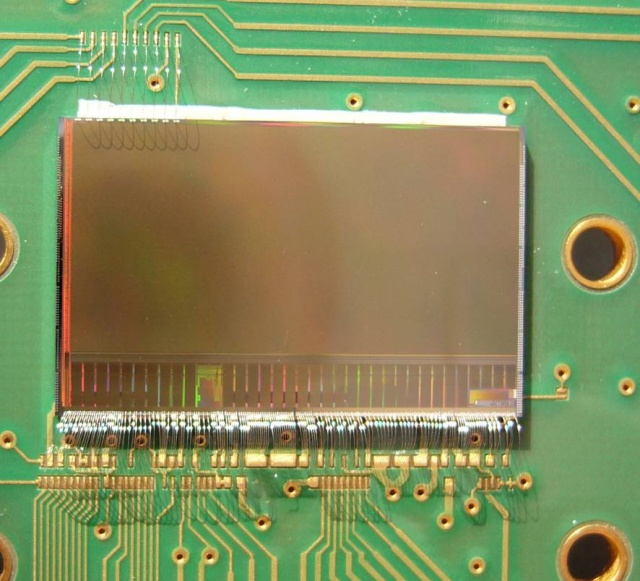
\includegraphics[width=0.95\textwidth]{Pictures/vxd/mi26.jpg}
        \caption{Picture of a MIMOSA-26 mounted on a PCB.}
        \label{fig:mi26}
    \end{subfigure}
    \qquad
     %add desired spacing between images, e. g. ~, \quad, \qquad, \hfill etc. 
      %(or a blank line to force the subfigure onto a new line)
    \begin{subfigure}[t]{0.4\textwidth}
        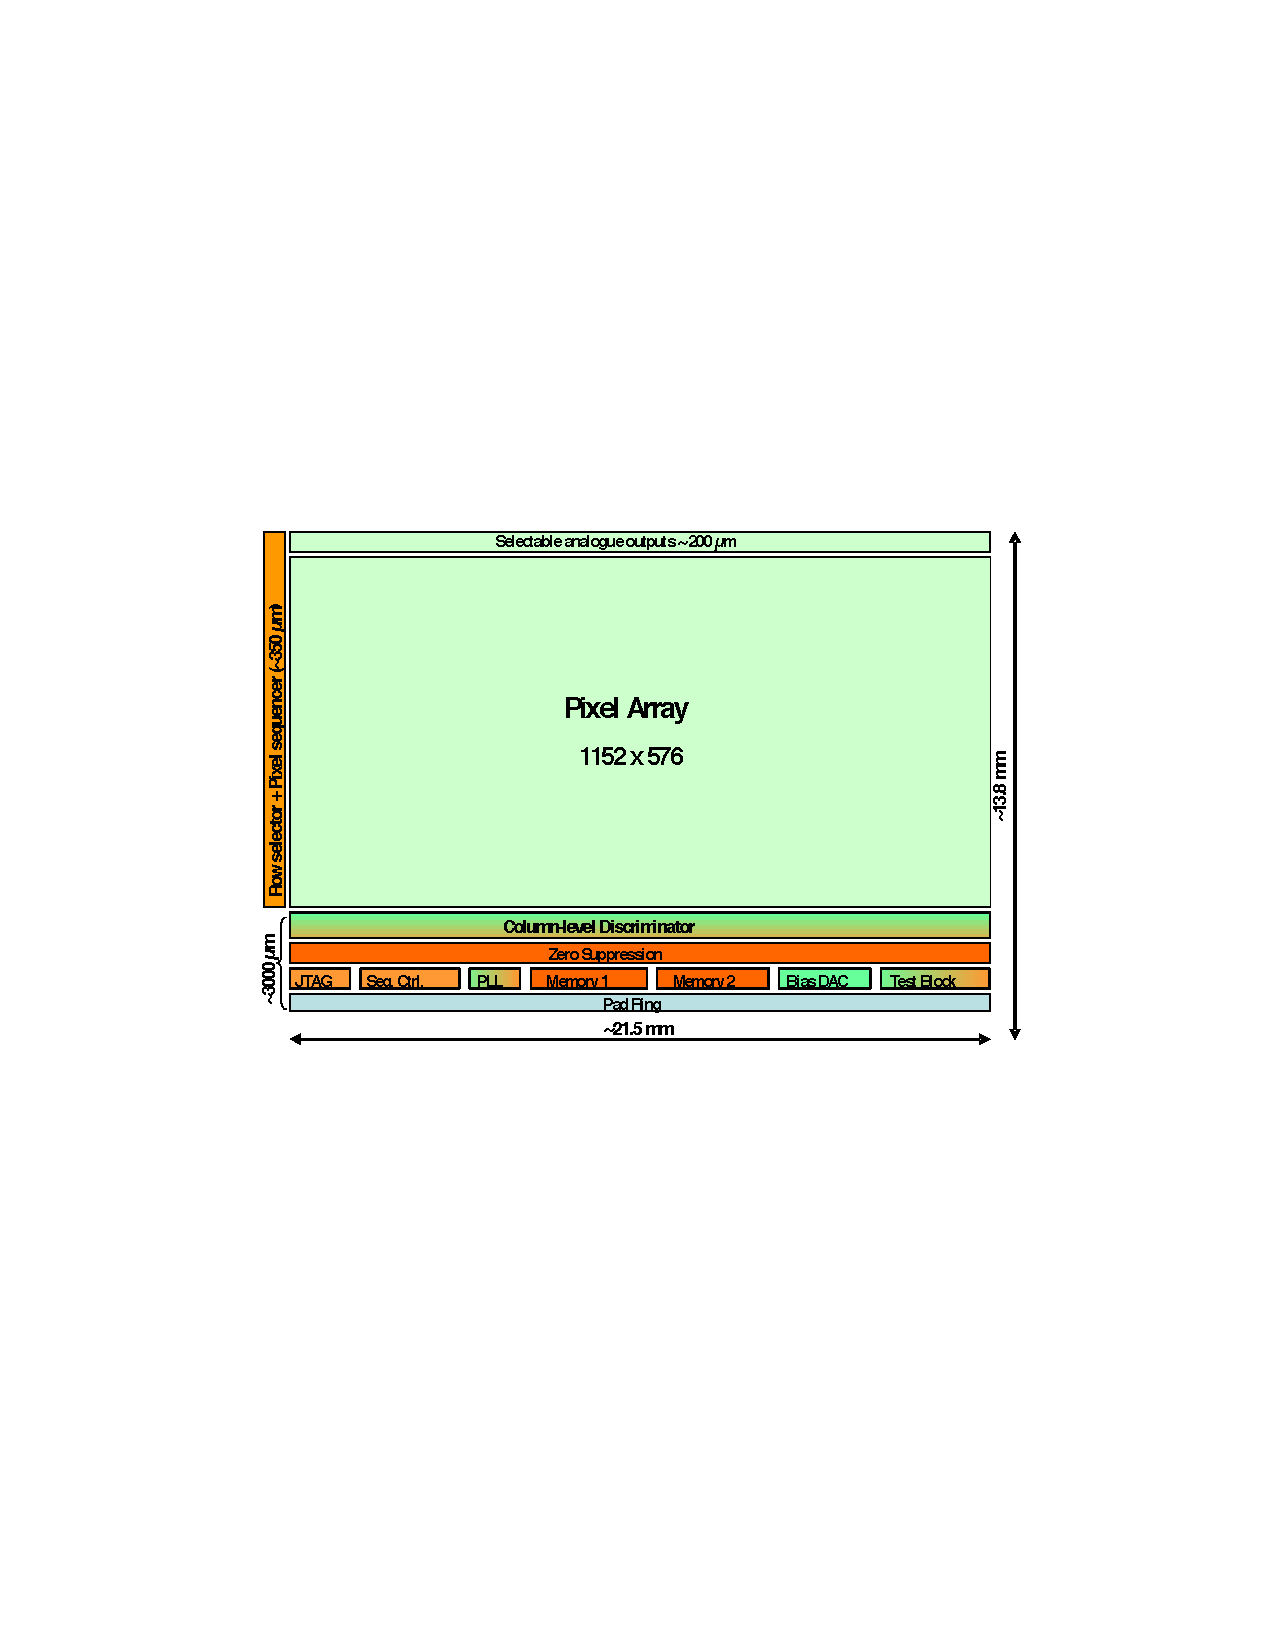
\includegraphics[width=1.35\textwidth]{Pictures/vxd/mi26_architecture.pdf}
        \caption{Layout of the MIMOSA-26 matrix.}
        \label{fig:archMi26}
    \end{subfigure}
    \caption{Block-diagram and a picture of the MIMOSA-26}\label{fig:Mi26}
    \end{figure}    



    The PICSEL group has then developed digital output sensors for the pixel vertex detector at the START experiment at Brookhaven National Laboratory\cite{}.
    The figure~\ref{fig:Mi28} is showing a half-section of the STAR vertex detector (subfigure~\ref{fig:vxdSTAR}) and a \gls{MIMOSA}-28 bounded on a PCB(subfigure~\ref{fig:ultimate}).
    They are based on the architecture of \gls{MIMOSA}-26 with some modifications.
    The matrix contains 960 columns and 928 rows for a pitch of $20.7 \times 20.7 \mu\text{m}^2$.
    The sensitive area is 19.7 x 19.2 $\text{cm}^2$, for an integration time of less than $200\mu\text{s}$.
    The sensor can reach a particle detection rate of $10^6$ particles/$\text{cm}^2$/s. 
    Finally, their power consumption is lower or equal to 150 mW/$\text{cm}^2$.
    The spatial resolution obtained for ULTIMATE is less than 4 $\mu\text{m}$.

  

    %The PICSEL group has developed sensors, called ULTIMATE, for the STAR experiment at Brookhaven National Laboratory\todo{REF to a paper}.
    %They are based on \gls{MIMOSA}-28 sensors and are integrated into the vertex detector.
    %The choice for this technology was made because of their characteristics.
    %Indeed, the thickness of a sensor is around 50 $\mu\text{m}$ in order to minimise the multiple scattering of particles.
    %The matrix is made of roughly $9 \times 10^5$ pixels, corresponding to 960 columns and 928 rows for a pitch of 20.7 x 20.7 $\mu\text{m}^2$.
    %The sensitive area is 19.7 x 19.2 $\text{cm}^2$.
    %They have a binary output integrating a zero suppression technology (SUZE) and the integration time of the whole matrix is 200 $\mu\text{s}$.
    %Thanks to this architecture, the sensors can reach a particle detection rate of $10^6$ particles/$\text{cm}^2$/s. 
    %Finally, their power consumption is lower or equal to 150 mW/$\text{cm}^2$.
    %The spatial resolution obtained for ULTIMATE is less than 4 $\mu\text{m}$.

  \begin{figure}[!h]
    \centering
    \begin{subfigure}[t]{0.4\textwidth}
        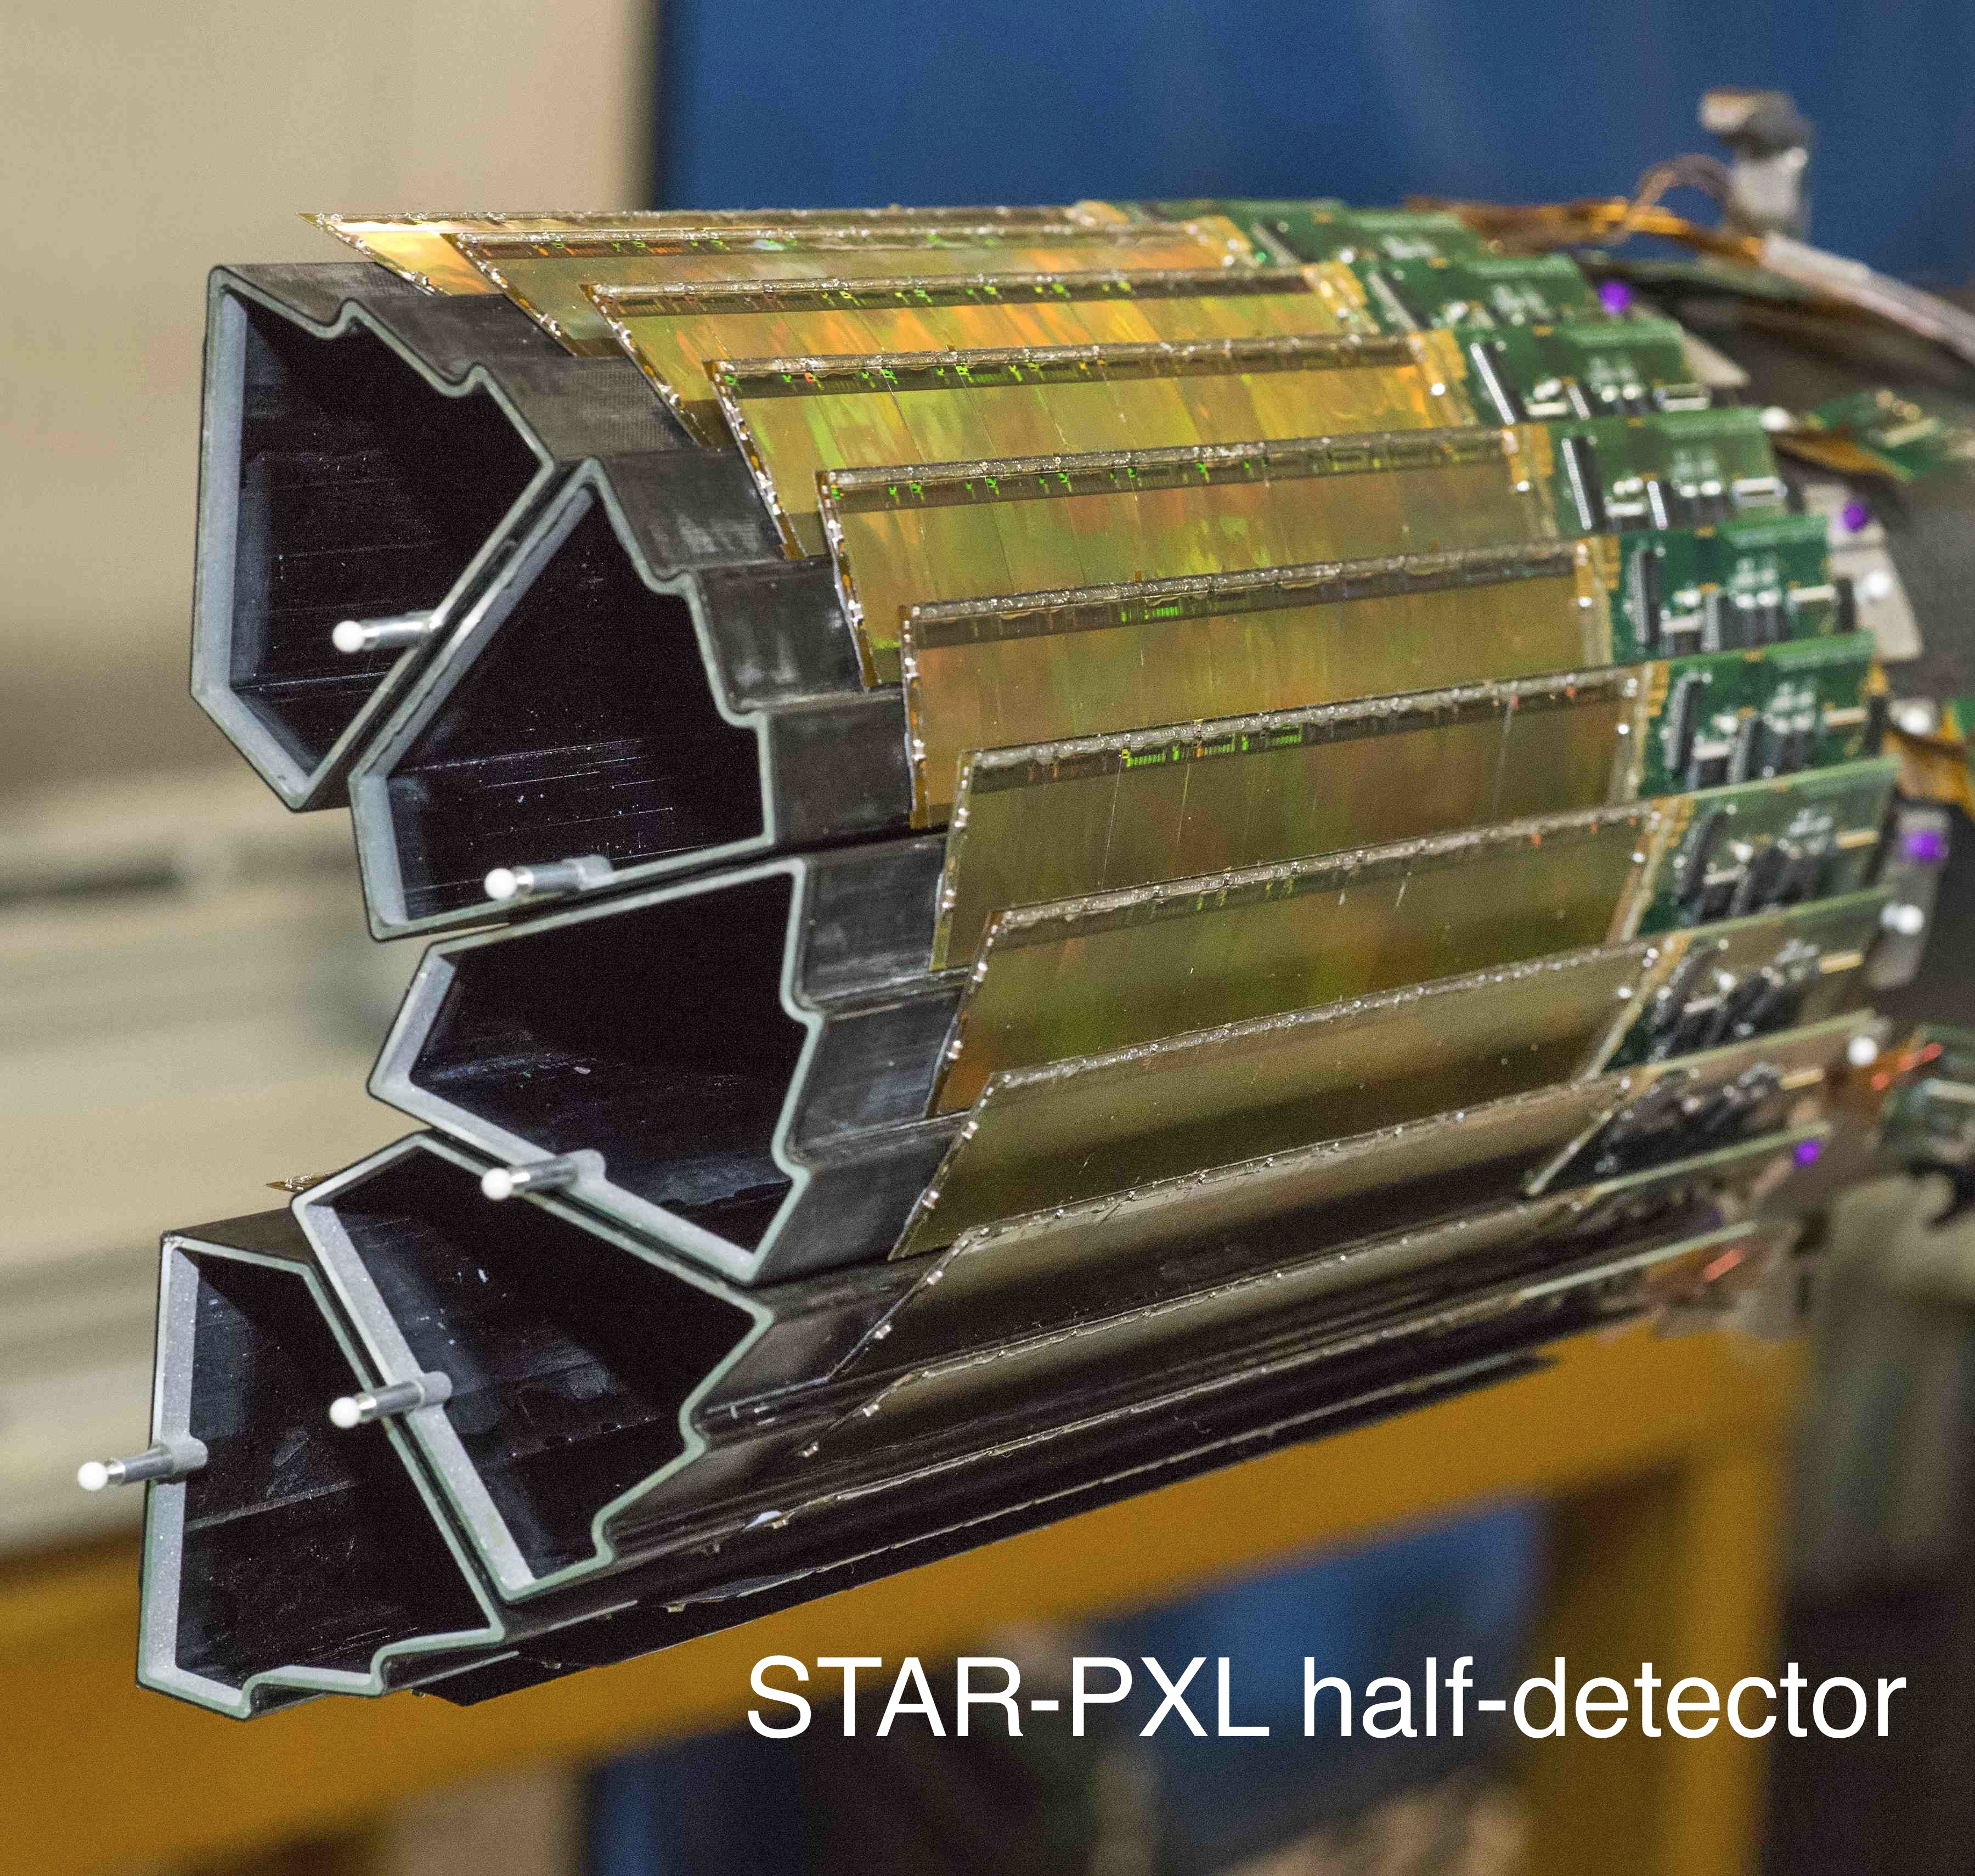
\includegraphics[width=\textwidth]{Pictures/vxd/pxlFinal_sideView_smallSize.jpg}
        \caption{Half part picture of the pixel vertex detector at STAR.}
        \label{fig:vxdSTAR}
    \end{subfigure}
    \qquad
     %add desired spacing between images, e. g. ~, \quad, \qquad, \hfill etc. 
      %(or a blank line to force the subfigure onto a new line)
    \begin{subfigure}[t]{0.4\textwidth}
        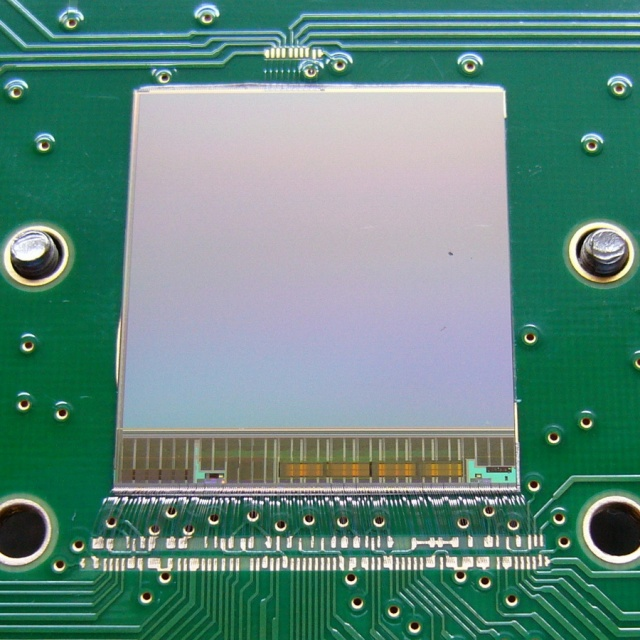
\includegraphics[width=0.95\textwidth]{Pictures/vxd/ultimate2.jpg}
        \caption{ULTIMATE chip mounted on a PCB. %The top wire bounds are used for a slow analog output dedicated to lab test, while the bottom ones are the wire bounds which control and read the sensor. }
        }
        \label{fig:ultimate}
    \end{subfigure}
    \caption{Pictures of the STAR vertex detector and an ULTIMATE chip}\label{fig:Mi28}
    \end{figure}    


    This chapter has depicted the purpose of the vertex detector for the \gls{ILD}.
    Different technologies were introduced, to focus specifically on the \gls{CMOS} sensors and their use in high-energy physics.
    The \gls{PLUME} collaboration aims to integrate \gls{MAPS} onto light double-sided ladders, in order to reach the requirements of the \gls{ILC}.
    The collaboration has reach different steps to produce the first full-scale ladder, which have only a material budget of only $0.35\% X_0$ and a spatial resolution better than $4\mu\text{m}$.
    The principle of the \gls{CMOS} technology was presented. 
    The next chapter is focusing on the electrical validation of this sensors mounted onto a PLUME ladder.

    


